\documentclass[11pt]{article}

\usepackage{fontspec}
\setmainfont{TeX Gyre Heros}
\setmonofont{TeX Gyre Cursor}[Scale=0.86]
\usepackage[a4paper,margin=2cm,top=1.8cm,bottom=1.8cm]{geometry}
\usepackage{tikz}
\usetikzlibrary{arrows.meta,positioning,shapes.geometric,calc,fit,backgrounds,decorations.pathreplacing}
\usepackage{xcolor}
\usepackage[most]{tcolorbox}
\usepackage{enumitem}
\usepackage{titlesec}
\usepackage{array}
\usepackage{booktabs}
\usepackage{amssymb}
\usepackage{fancyhdr}
\usepackage{hyperref}

% ---------- palette ----------
\definecolor{ink}{HTML}{18212F}
\definecolor{muted}{HTML}{5B6779}
\definecolor{accent}{HTML}{2563EB}
\definecolor{accentlt}{HTML}{DBEAFE}
\definecolor{good}{HTML}{047857}
\definecolor{goodlt}{HTML}{D1FAE5}
\definecolor{bad}{HTML}{B91C1C}
\definecolor{badlt}{HTML}{FEE2E2}
\definecolor{warn}{HTML}{B45309}
\definecolor{warnlt}{HTML}{FEF3C7}
\definecolor{paper}{HTML}{F8FAFC}
\definecolor{line}{HTML}{CBD5E1}

\color{ink}

\hypersetup{colorlinks=true,linkcolor=accent,urlcolor=accent}

% ---------- headings ----------
\titleformat{\section}{\LARGE\bfseries\color{ink}}{\thesection.}{0.4em}{}
\titlespacing*{\section}{0pt}{18pt}{8pt}
\titleformat{\subsection}{\large\bfseries\color{accent}}{}{0em}{}
\titlespacing*{\subsection}{0pt}{12pt}{4pt}

\setlength{\parindent}{0pt}
\setlength{\parskip}{6pt}

\pagestyle{fancy}\fancyhf{}
\renewcommand{\headrulewidth}{0pt}
\fancyfoot[C]{\small\color{muted}Prior art review — issue \#175 — 6 August 2026 — page \thepage}

% ---------- helpers ----------
\newcommand{\code}[1]{{\small\texttt{#1}}}
\newcommand{\shout}[1]{\textbf{#1}}

\newtcolorbox{keybox}[1]{
  enhanced, colback=accentlt, colframe=accent, boxrule=0pt, leftrule=3pt,
  arc=2pt, left=10pt,right=10pt,top=8pt,bottom=8pt,
  title={\bfseries #1}, coltitle=accent, fonttitle=\bfseries,
  attach boxed title to top left={xshift=10pt,yshift=-2pt},
  boxed title style={colback=accentlt,boxrule=0pt,arc=0pt}
}
\newtcolorbox{badbox}[1]{
  enhanced, colback=badlt, colframe=bad, boxrule=0pt, leftrule=3pt,
  arc=2pt, left=10pt,right=10pt,top=8pt,bottom=8pt,
  title={\bfseries #1}, coltitle=bad, fonttitle=\bfseries,
  attach boxed title to top left={xshift=10pt,yshift=-2pt},
  boxed title style={colback=badlt,boxrule=0pt,arc=0pt}}
\newtcolorbox{goodbox}{
  enhanced, colback=goodlt, colframe=good, boxrule=0pt, leftrule=3pt,
  arc=2pt, left=10pt,right=10pt,top=8pt,bottom=8pt}
\newtcolorbox{plainbox}{
  enhanced, colback=paper, colframe=line, boxrule=0.6pt,
  arc=2pt, left=10pt,right=10pt,top=8pt,bottom=8pt}

\tikzset{
  box/.style={draw=line, fill=white, rounded corners=3pt, align=center,
              font=\small, inner sep=6pt, thick},
  bluebox/.style={box, fill=accentlt, draw=accent},
  redbox/.style={box, fill=badlt, draw=bad},
  greenbox/.style={box, fill=goodlt, draw=good},
  warnbox/.style={box, fill=warnlt, draw=warn},
  ar/.style={-{Stealth[length=6pt]}, thick, draw=muted},
  arred/.style={-{Stealth[length=6pt]}, thick, draw=bad},
  argreen/.style={-{Stealth[length=6pt]}, thick, draw=good},
  lbl/.style={font=\scriptsize\itshape, color=muted}
}

\begin{document}

% =====================================================================
\begin{center}
{\Huge\bfseries What ten other projects\\[4pt] already know}\\[10pt]
{\large\color{muted} A plain-language summary of the prior-art review (issue \#175)}\\[4pt]
{\small\color{muted} 6 August 2026 \quad$\cdot$\quad ten repositories read at pinned commits \quad$\cdot$\quad nine test suites actually run}
\end{center}

\vspace{6pt}

\begin{keybox}{The one-paragraph version}
We read the ten public projects that are built most like mcgyvr, at exact
commits, and \emph{ran their tests} rather than trusting their READMEs. Then six
independent readers checked the first pass. The most useful things we found were
not clever features --- they were \shout{mistakes these projects made and paid
for}. Four of them are mistakes mcgyvr is currently positioned to repeat, and
\shout{one of them mcgyvr has already made}: our capacity limit doesn't work
across processes, and our own workflow runs multiple processes.
\end{keybox}

\vspace{-2pt}

\subsection*{The scoreboard}

\begin{center}
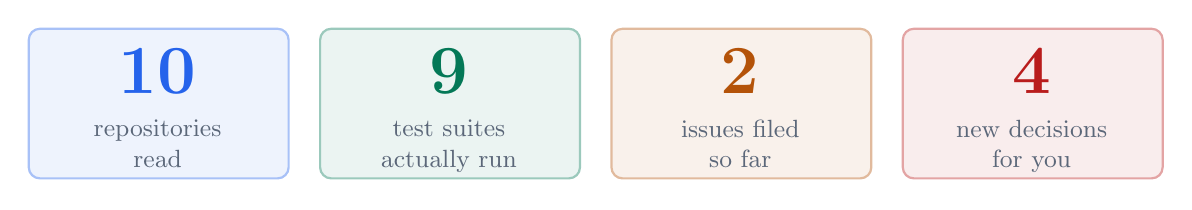
\begin{tikzpicture}[node distance=0pt]
  \foreach \x/\num/\lab/\col in {
     0/10/repositories\\read/accent,
     3.7/9/test suites\\actually run/good,
     7.4/2/issues filed\\so far/warn,
     11.1/4/new decisions\\for you/bad} {
    \node[anchor=north west, minimum width=3.3cm, minimum height=1.9cm,
          rounded corners=4pt, fill=\col!8, draw=\col!40, thick] at (\x,0) {};
    \node[anchor=north] at (\x+1.65,-0.15) {\fontsize{30}{30}\selectfont\bfseries\color{\col}\num};
    \node[anchor=north, align=center, font=\small\color{muted}] at (\x+1.65,-1.05) {\lab};
  }
\end{tikzpicture}
\end{center}

\begin{plainbox}
\shout{Why "actually run" matters.} A project's README says what its author
hoped. Its tests say what its author was burned by. We only counted a finding if
we could point at code at a specific commit, or run something. The first pass
said four test suites "couldn't be run here" --- \shout{three of those four ran
fine on a second attempt}. That is a lesson about us, not about them.
\end{plainbox}

\newpage
% =====================================================================
\section{First, the map: who sits where}

The most important decision in this review was \emph{which} projects to read. It
turns out there are two very different kinds of tool, and most famous ones are
the wrong kind for us to learn from.

\begin{center}
\resizebox{\textwidth}{!}{%
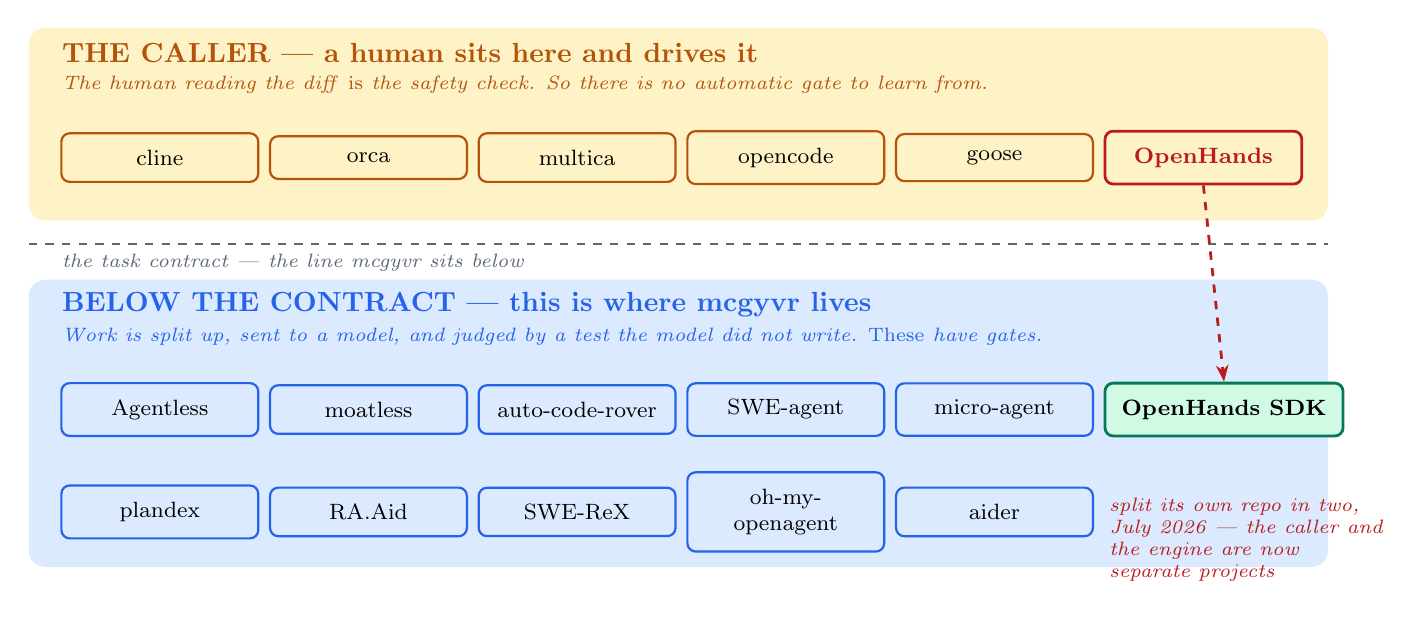
\begin{tikzpicture}[x=1cm,y=1cm]

  % top band
  \fill[warnlt, rounded corners=6pt] (-0.25,2.25) rectangle (16.25,4.7);
  \node[anchor=west, font=\bfseries\color{warn}] at (0.05,4.38) {THE CALLER --- a human sits here and drives it};
  \node[anchor=west, font=\scriptsize\itshape\color{warn}] at (0.05,3.98)
      {The human reading the diff \emph{is} the safety check. So there is no automatic gate to learn from.};
  \foreach \x/\n in {0.15/cline, 2.8/orca, 5.45/multica, 8.1/opencode, 10.75/goose} {
     \node[warnbox, anchor=west, minimum width=2.5cm, font=\footnotesize] at (\x,3.05) {\n};
  }
  \node[warnbox, anchor=west, minimum width=2.5cm, font=\footnotesize,
        draw=bad, line width=1pt] (oh) at (13.4,3.05) {\color{bad}\bfseries OpenHands};

  % divider
  \draw[dashed, thick, muted] (-0.25,1.95) -- (16.25,1.95);
  \node[anchor=west, lbl] at (0.05,1.72) {the task contract --- the line mcgyvr sits below};

  % bottom band
  \fill[accentlt, rounded corners=6pt] (-0.25,-2.15) rectangle (16.25,1.5);
  \node[anchor=west, font=\bfseries\color{accent}] at (0.05,1.18) {BELOW THE CONTRACT --- this is where mcgyvr lives};
  \node[anchor=west, font=\scriptsize\itshape\color{accent}] at (0.05,0.78)
      {Work is split up, sent to a model, and judged by a test the model did not write. \emph{These} have gates.};
  \foreach \x/\n in {0.15/Agentless, 2.8/moatless, 5.45/{auto-code-rover}, 8.1/{SWE-agent}, 10.75/{micro-agent}} {
     \node[bluebox, anchor=west, minimum width=2.5cm, font=\footnotesize] at (\x,-0.15) {\n};
  }
  \node[greenbox, anchor=west, minimum width=2.5cm, font=\footnotesize,
        line width=1pt] (sdk) at (13.4,-0.15) {\bfseries OpenHands SDK};
  \foreach \x/\n in {0.15/plandex, 2.8/RA.Aid, 5.45/{SWE-ReX}, 8.1/{oh-my-\\openagent}, 10.75/aider} {
     \node[bluebox, anchor=west, minimum width=2.5cm, font=\footnotesize] at (\x,-1.45) {\n};
  }

  % the split
  \draw[arred, dashed, line width=1pt] (oh.south) -- (sdk.north);
  \node[anchor=north west, align=left, font=\scriptsize\itshape, color=bad] at (13.35,-1.15)
      {split its own repo in two,\\July 2026 --- the caller and\\the engine are now\\separate projects};
\end{tikzpicture}}
\end{center}

\begin{goodbox}
\shout{The best thing we found all week.} Ten days before we looked, OpenHands ---
the biggest project of this type, 83,000 stars --- \shout{split its repository in
half along exactly this line}. One repo is now the caller; the other is the
engine underneath. We drew that line from theory. They drew it in production and
deleted 486,115 lines doing it. That is independent confirmation that the line is
real.
\end{goodbox}

\newpage
% =====================================================================
\section{Finding 1: a test needs its own check}

Every one of these systems asks a model to write a test that proves the bug is
fixed. And \shout{not one of them trusts that test}. Each invented a different
way to check the checker:

\begin{center}
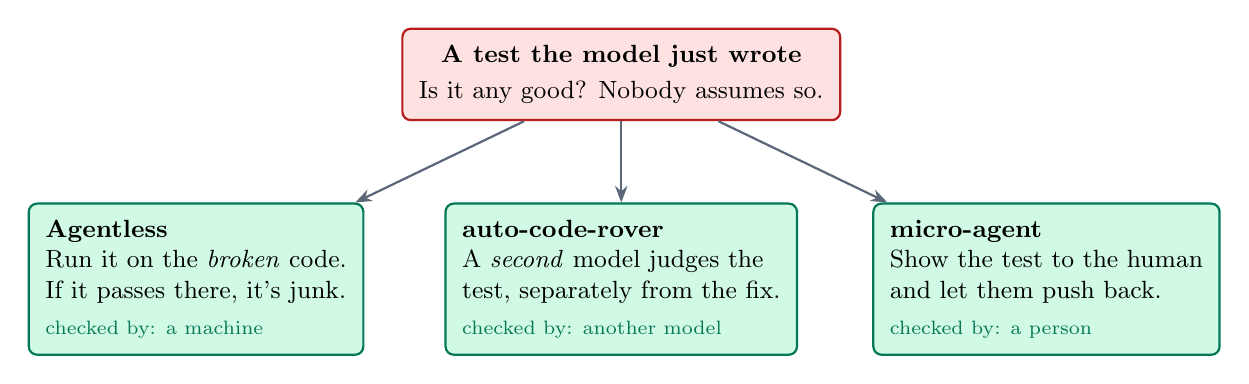
\begin{tikzpicture}[x=1cm,y=1cm]
  \node[redbox, minimum width=4.6cm] (t) at (7,0) {\bfseries A test the model just wrote\\[2pt]\small Is it any good? Nobody assumes so.};

  \node[greenbox, minimum width=4.1cm, align=left] (a) at (1.6,-2.6)
     {\bfseries Agentless\\\small Run it on the \emph{broken} code.\\\small If it passes there, it's junk.\\[2pt]\scriptsize\color{good}checked by: a machine};
  \node[greenbox, minimum width=4.1cm, align=left] (b) at (7,-2.6)
     {\bfseries auto-code-rover\\\small A \emph{second} model judges the\\\small test, separately from the fix.\\[2pt]\scriptsize\color{good}checked by: another model};
  \node[greenbox, minimum width=4.1cm, align=left] (c) at (12.4,-2.6)
     {\bfseries micro-agent\\\small Show the test to the human\\\small and let them push back.\\[2pt]\scriptsize\color{good}checked by: a person};

  \draw[ar] (t) -- (a); \draw[ar] (t) -- (b); \draw[ar] (t) -- (c);
\end{tikzpicture}
\end{center}

\subsection*{And when the checker itself breaks?}

That is the question mcgyvr has open (\#179): if the reviewer crashes, is that the
\emph{work's} fault or the \emph{reviewer's} fault? Two projects shipped an answer
and they agree; one disagrees. This is a real fork in the road, and you have to pick.

\begin{center}
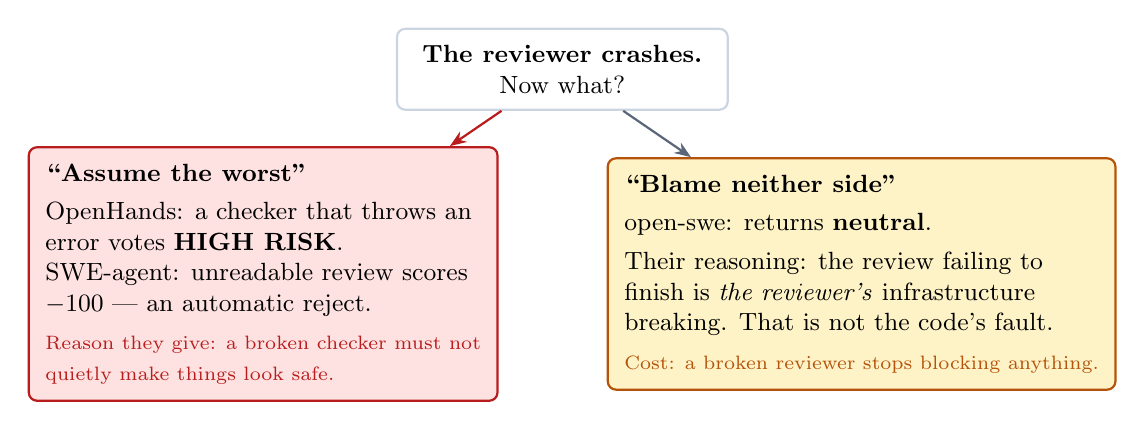
\begin{tikzpicture}[x=1cm,y=1cm]
  \node[box, minimum width=4.2cm] (q) at (7.2,0.4) {\bfseries The reviewer crashes.\\Now what?};
  \node[redbox, minimum width=5.4cm, align=left] (fc) at (3.4,-2.2)
    {\bfseries ``Assume the worst''\\[3pt]\small OpenHands: a checker that throws an\\\small error votes \shout{HIGH RISK}.\\
     \small SWE-agent: unreadable review scores\\\small $-100$ --- an automatic reject.\\[3pt]
     \scriptsize\color{bad} Reason they give: a broken checker must not\\\scriptsize\color{bad} quietly make things look safe.};
  \node[warnbox, minimum width=5.4cm, align=left] (nu) at (11.0,-2.2)
    {\bfseries ``Blame neither side''\\[3pt]\small open-swe: returns \shout{neutral}.\\[3pt]
     \small Their reasoning: the review failing to\\\small finish is \emph{the reviewer's} infrastructure\\\small breaking. That is not the code's fault.\\[3pt]
     \scriptsize\color{warn} Cost: a broken reviewer stops blocking anything.};
  \draw[arred] (q) -- (fc); \draw[ar] (q) -- (nu);
\end{tikzpicture}
\end{center}

\begin{keybox}{What this means for you}
You don't need to invent an answer to \#179 --- you need to \emph{choose} between
two that already exist and have been run in anger. "Fail closed" is safer and
noisier. "Neutral" keeps the pipeline moving and lets a broken reviewer wave
things through.
\end{keybox}

\newpage
% =====================================================================
\section{Finding 2: the scariest thing we found}

RA.Aid has a safety gate: you give it a test command, and it runs your tests
before accepting the model's work. \shout{That gate has not run since 27 January
2025.} It crashes instantly, every time, on a typo-level bug --- it passes an
argument the function doesn't accept.

That alone would be bad. Here is what makes it genuinely dangerous:

\begin{center}
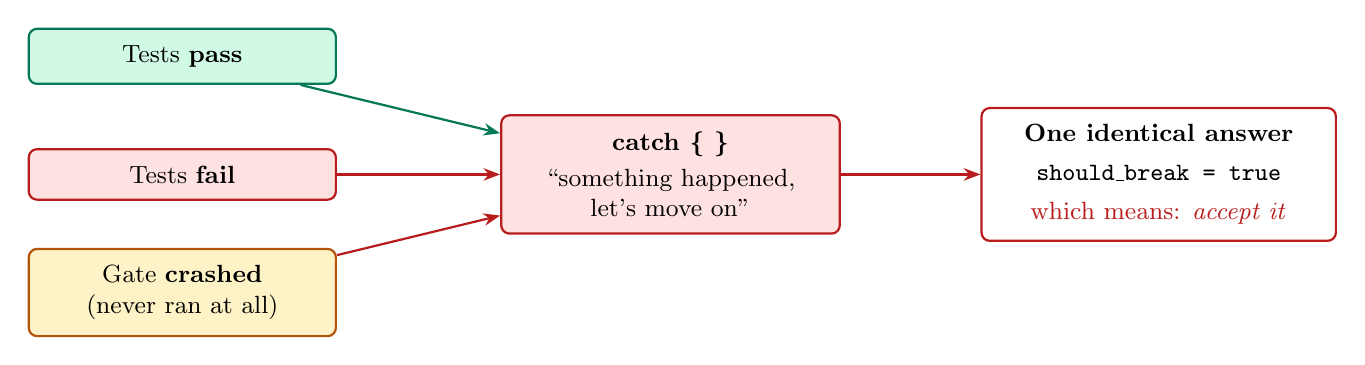
\begin{tikzpicture}[x=1cm,y=1cm]
  \node[greenbox, minimum width=3.9cm] (g) at (0.6,1.5) {Tests \shout{pass}};
  \node[redbox,   minimum width=3.9cm] (r) at (0.6,0.0) {Tests \shout{fail}};
  \node[warnbox,  minimum width=3.9cm] (x) at (0.6,-1.5) {Gate \shout{crashed}\\\small(never ran at all)};

  \node[box, draw=bad, fill=badlt, minimum width=4.3cm, align=center] (c) at (6.8,0)
      {\bfseries catch \{ \} \\[2pt]\small ``something happened,\\\small let's move on''};

  \node[box, draw=bad, fill=white, minimum width=4.5cm, align=center] (o) at (13.0,0)
      {\bfseries One identical answer\\[3pt]\code{should\_break = true}\\[3pt]\small\color{bad} which means: \emph{accept it}};

  \draw[argreen] (g) -- (c);
  \draw[arred] (r) -- (c);
  \draw[arred] (x) -- (c);
  \draw[arred, line width=1.2pt] (c) -- (o);
\end{tikzpicture}
\end{center}

Three completely different situations --- everything worked, everything is broken,
the check never happened --- come out the other side as \shout{the same single
value}. Nothing downstream can tell them apart. We verified this by running their
own code three ways.

\begin{badbox}{And this is why nobody noticed}
The gate has six tests. All six pass. They pass because each one
\shout{replaces the real function with a fake} that politely accepts any
argument --- including the argument that breaks the real one.

\medskip
\emph{The mock is the thing that kept it green for eighteen months.}
\end{badbox}

\begin{center}
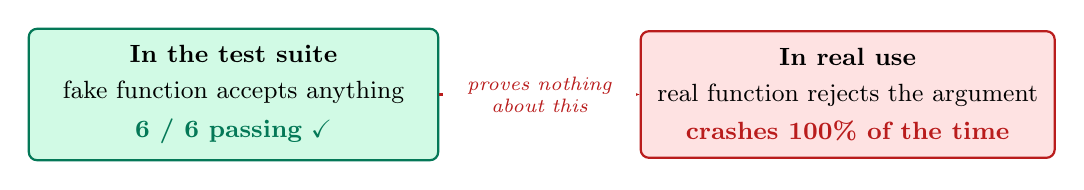
\begin{tikzpicture}[x=1cm,y=1cm]
  \node[greenbox, minimum width=5.2cm, align=center] (t) at (3.2,0) {\bfseries In the test suite\\[2pt]\small fake function accepts anything\\[3pt]\small\color{good}\shout{6 / 6 passing} \checkmark};
  \node[redbox, minimum width=5.2cm, align=center] (p) at (11.0,0) {\bfseries In real use\\[2pt]\small real function rejects the argument\\[3pt]\small\color{bad}\shout{crashes 100\% of the time}};
  \draw[arred, dashed, line width=1pt] (t) -- node[lbl, color=bad, align=center, text width=2.3cm, fill=white, inner sep=2pt] {proves nothing\\about this} (p);
\end{tikzpicture}
\end{center}

\begin{keybox}{The question this puts to mcgyvr}
Two things, both narrow enough to answer today:
\begin{enumerate}[leftmargin=16pt, itemsep=2pt]
  \item Should the piece of mcgyvr that \emph{actually shells out to run the
        tests} be allowed to be faked in \emph{any} test? RA.Aid says no,
        expensively.
  \item Can a yes/no value carry \emph{passed}, \emph{failed} \shout{and}
        \emph{never ran}? It cannot. Right now we have two of those three
        sharing a slot.
\end{enumerate}
\end{keybox}

\newpage
% =====================================================================
\section{Finding 3: saved model replies rot --- unless you save the right part}

We have an open idea (\#184) to start saving what the models say back to us,
since we already have it and throw it away. Good idea, but OpenHands did exactly
that and it died within a week. Here is the timeline:

\begin{center}
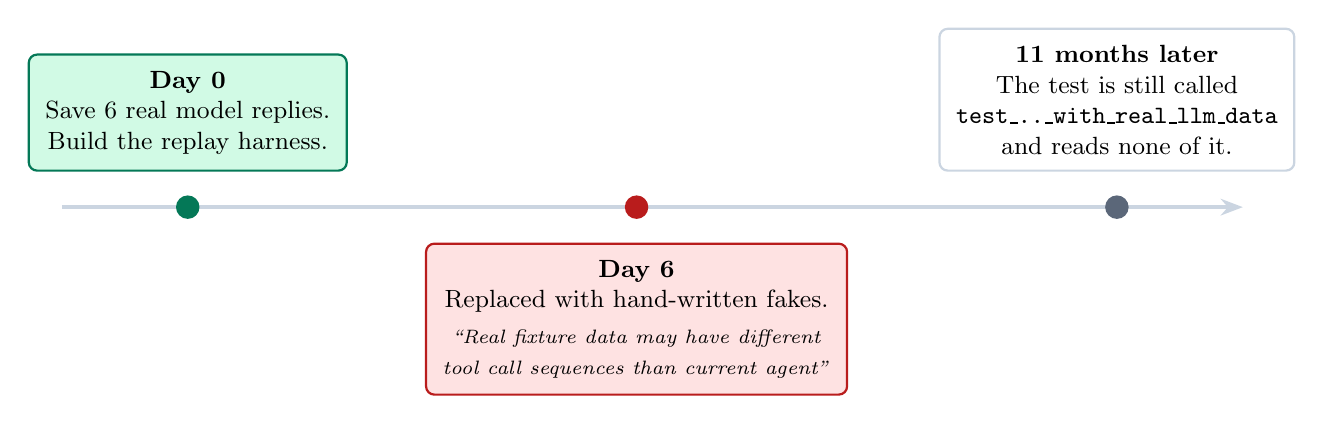
\begin{tikzpicture}[x=1cm,y=1cm]
  \draw[line width=1.5pt, line, -{Stealth[length=8pt]}] (0,0) -- (15,0);

  \node[circle, fill=good, inner sep=3pt] at (1.6,0) {};
  \node[greenbox, anchor=south, minimum width=3.9cm] at (1.6,0.45)
     {\bfseries Day 0\\\small Save 6 real model replies.\\\small Build the replay harness.};

  \node[circle, fill=bad, inner sep=3pt] at (7.3,0) {};
  \node[redbox, anchor=north, minimum width=5.0cm] at (7.3,-0.45)
     {\bfseries Day 6\\\small Replaced with hand-written fakes.\\[2pt]\scriptsize\emph{``Real fixture data may have different}\\\scriptsize\emph{tool call sequences than current agent''}};

  \node[circle, fill=muted, inner sep=3pt] at (13.4,0) {};
  \node[box, anchor=south, minimum width=4.4cm] at (13.4,0.45)
     {\bfseries 11 months later\\\small The test is still called\\\code{test\_..\_with\_real\_llm\_data}\\\small and reads none of it.};
\end{tikzpicture}
\end{center}

\subsection*{Why it rotted, and what to save instead}

\begin{center}
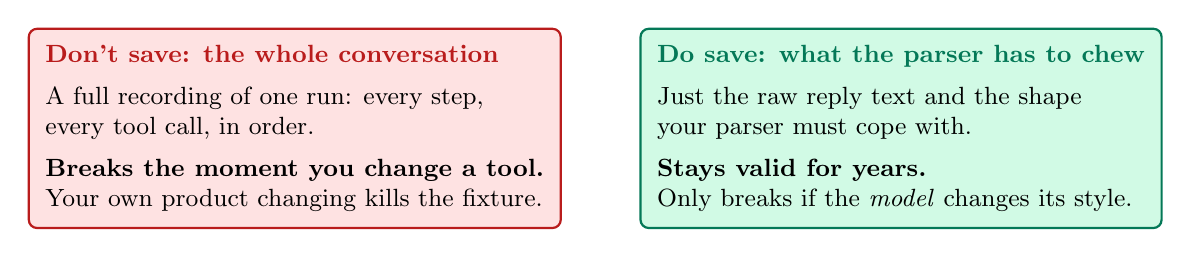
\begin{tikzpicture}[x=1cm,y=1cm]
  \node[redbox, minimum width=6.6cm, align=left] (a) at (3.9,0)
    {\bfseries \color{bad}Don't save: the whole conversation\\[4pt]
     \small A full recording of one run: every step,\\\small every tool call, in order.\\[4pt]
     \small\shout{Breaks the moment you change a tool.}\\
     \small Your own product changing kills the fixture.};
  \node[greenbox, minimum width=6.6cm, align=left] (b) at (11.6,0)
    {\bfseries \color{good}Do save: what the parser has to chew\\[4pt]
     \small Just the raw reply text and the shape\\\small your parser must cope with.\\[4pt]
     \small\shout{Stays valid for years.}\\
     \small Only breaks if the \emph{model} changes its style.};
\end{tikzpicture}
\end{center}

aider is the proof of the good version: \shout{99,961 lines} of real captured
replies, checked against a reference file --- and crucially it keeps
\shout{33 replies that failed to parse}, as treasured examples rather than
embarrassments. That corpus cost them one \code{git add} of a log they already had.

\begin{keybox}{What this means for you}
\#184 is right, but it should be reworded before anyone builds it: capture
\shout{what the parser reads}, not \shout{what the run did}. Same effort,
one lasts and one doesn't.
\end{keybox}

\newpage
% =====================================================================
\section{Finding 4: limits that lie about why they stopped}

SWE-agent looks exemplary here. It has four separate spending limits, each with
its own name, so a run can always say why it gave up. Except it can't:

\begin{center}
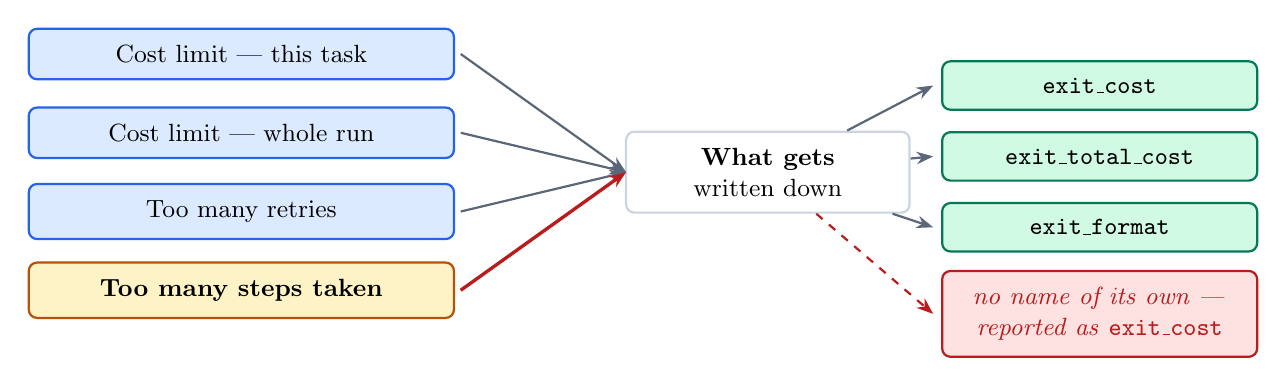
\begin{tikzpicture}[x=1cm,y=1cm]
  \foreach \y/\n in {2.4/{Cost limit --- this task}, 1.4/{Cost limit --- whole run}, 0.4/{Too many retries}} {
    \node[bluebox, anchor=west, minimum width=5.4cm] at (0,\y) {\n};
  }
  \node[warnbox, anchor=west, minimum width=5.4cm] at (0,-0.6) {\bfseries Too many steps taken};

  \node[box, minimum width=3.6cm, align=center] (m) at (9.4,0.9) {\bfseries What gets\\written down};

  \foreach \y in {2.4,1.4,0.4} { \draw[ar] (5.5,\y) -- (7.6,0.9); }
  \draw[arred, line width=1.2pt] (5.5,-0.6) -- (7.6,0.9);

  \node[greenbox, anchor=west, minimum width=4.0cm] at (11.6,2.0) {\code{exit\_cost}};
  \node[greenbox, anchor=west, minimum width=4.0cm] at (11.6,1.1) {\code{exit\_total\_cost}};
  \node[greenbox, anchor=west, minimum width=4.0cm] at (11.6,0.2) {\code{exit\_format}};
  \node[redbox, anchor=west, minimum width=4.0cm, align=center] at (11.6,-0.9) {\small\color{bad}\emph{no name of its own ---}\\\small\color{bad}\emph{reported as} \code{exit\_cost}};

  \draw[ar] (m) -- (11.5,2.0); \draw[ar] (m) -- (11.5,1.1); \draw[ar] (m) -- (11.5,0.2);
  \draw[arred, dashed] (m) -- (11.5,-0.9);
\end{tikzpicture}
\end{center}

The "too many steps" limit was written as a \emph{kind of} cost limit, purely for
convenience in the code. The side effect: \shout{a run that ran out of steps
reports that it ran out of money}. Whoever reads that log later will tune the
wrong dial.

\begin{plainbox}
There's a second one in the same file. A loop says "stop after 3 retries" --- but
two of the ways it retries \shout{never increment the counter}. So the limit
you declared is not the limit that operates; the budget stops it eventually,
by accident.

\medskip
\shout{The rule worth stealing:} every path that burns an iteration must count
one, and every limit you declare needs its own name in the record.
\end{plainbox}

\newpage
% =====================================================================
\section{Finding 5: everyone picks models by name, nobody by evidence}

aider has measured more model behaviour than anyone in this field --- years of
public benchmark runs. So we expected its model routing to be driven by that
data. It isn't. \shout{Nothing reads it.}

\begin{center}
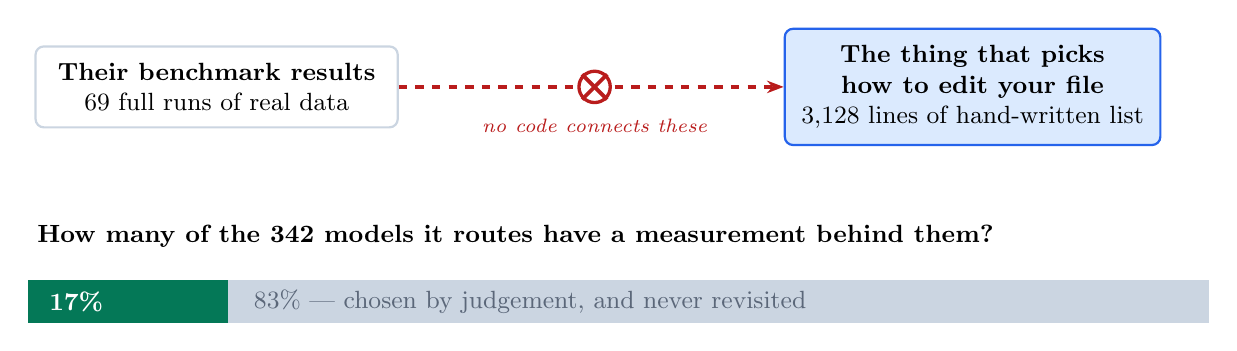
\begin{tikzpicture}[x=1cm,y=1cm]
  \node[box, minimum width=4.6cm, align=center] (lb) at (2.4,1.4)
      {\bfseries Their benchmark results\\\small 69 full runs of real data};
  \node[bluebox, minimum width=4.6cm, align=center] (rt) at (12.0,1.4)
      {\bfseries The thing that picks\\\bfseries how to edit your file\\\small 3,128 lines of hand-written list};

  \draw[arred, dashed, line width=1.4pt] (lb) -- (rt);
  \node[circle, draw=bad, fill=white, line width=1.2pt, inner sep=4pt] (x) at (7.2,1.4) {};
  \draw[bad, line width=1.4pt] ($(x)+(-0.16,-0.16)$) -- ($(x)+(0.16,0.16)$);
  \draw[bad, line width=1.4pt] ($(x)+(-0.16,0.16)$) -- ($(x)+(0.16,-0.16)$);
  \node[lbl, color=bad, below=2pt of x] {no code connects these};

  % coverage bar
  \node[anchor=west, font=\small\bfseries] at (0,-0.5) {How many of the 342 models it routes have a measurement behind them?};
  \fill[good] (0,-1.6) rectangle (2.55,-1.05);
  \fill[line] (2.55,-1.6) rectangle (15,-1.05);
  \node[anchor=west, font=\small\bfseries\color{white}] at (0.15,-1.33) {17\%};
  \node[anchor=west, font=\small\color{muted}] at (2.75,-1.33) {83\% --- chosen by judgement, and never revisited};
\end{tikzpicture}
\end{center}

\subsection*{The example that should matter most to you}

Their own published data, for exactly the class of model your rigs run:

\begin{center}
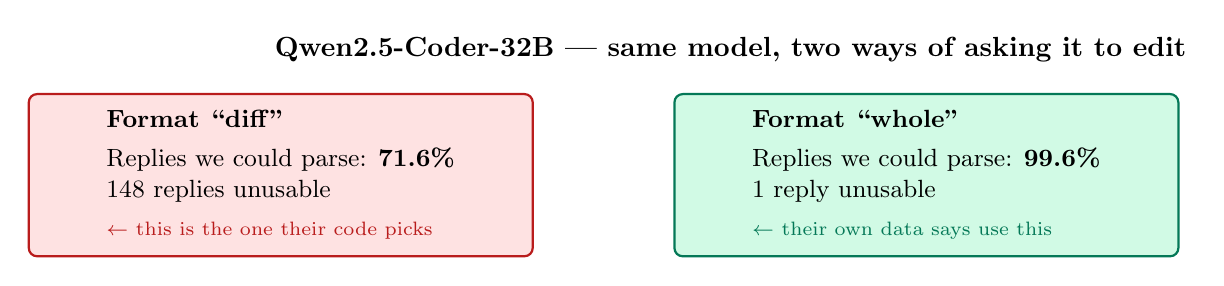
\begin{tikzpicture}[x=1cm,y=1cm]
  \node[anchor=west, font=\bfseries] at (0,0.7) {Qwen2.5-Coder-32B --- same model, two ways of asking it to edit};

  \node[redbox, minimum width=6.4cm, align=left] at (0.2,-0.9)
    {\bfseries Format ``diff''\\[3pt]\small Replies we could parse: \shout{71.6\%}\\\small 148 replies unusable\\[3pt]\scriptsize\color{bad}$\leftarrow$ this is the one their code picks};
  \node[greenbox, minimum width=6.4cm, align=left] at (8.4,-0.9)
    {\bfseries Format ``whole''\\[3pt]\small Replies we could parse: \shout{99.6\%}\\\small 1 reply unusable\\[3pt]\scriptsize\color{good}$\leftarrow$ their own data says use this};
\end{tikzpicture}
\end{center}

A 28-point swing in whether the model's answer is even \emph{usable}, from
changing nothing but how you ask. The weaker your model, the more this matters ---
and local models are the whole point of mcgyvr.

\begin{keybox}{What this means for you (\#162, the routing question)}
There is a cheap number nobody is using: \shout{what fraction of this worker's
replies did we manage to parse?} mcgyvr already produces it on every single
dispatch and throws it away. Routing on \emph{measured reply quality} instead of
\emph{model name} would be genuinely new --- nobody in this survey has built it.
\end{keybox}

\newpage
% =====================================================================
\section{Finding 6: the one that's about us}

This came out of the concurrency annex, and it is the most actionable thing in
the whole review.

mcgyvr limits how many jobs it sends to a machine at once. The limit is a counter
held \shout{inside one running process}. But the machines are shared, and your own
workflow runs \shout{several processes at the same time} --- that's what lanes in
separate worktrees are.

\begin{center}
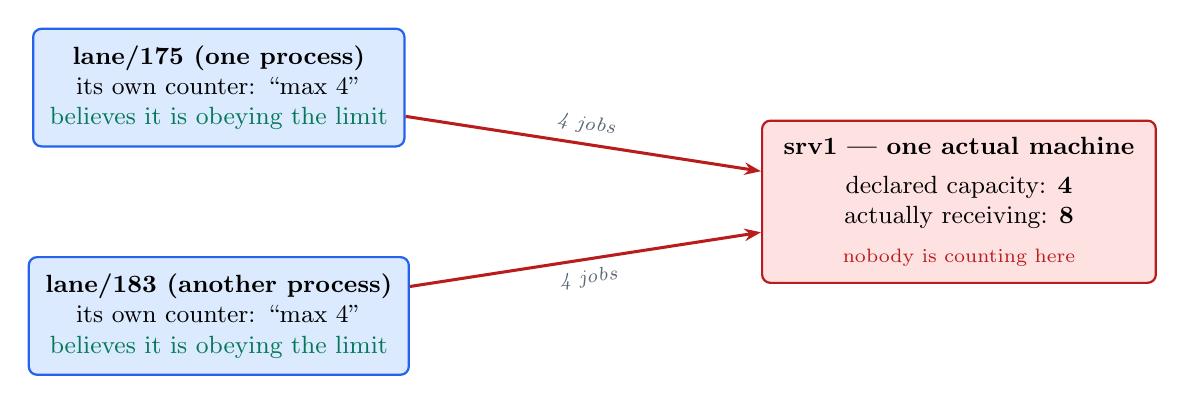
\begin{tikzpicture}[x=1cm,y=1cm]
  \node[bluebox, minimum width=4.4cm, align=center] (l1) at (2.6,1.9)
     {\bfseries lane/175 (one process)\\\small its own counter: ``max 4''\\\small\color{good}believes it is obeying the limit};
  \node[bluebox, minimum width=4.4cm, align=center] (l2) at (2.6,-1.0)
     {\bfseries lane/183 (another process)\\\small its own counter: ``max 4''\\\small\color{good}believes it is obeying the limit};

  \node[redbox, minimum width=5.0cm, align=center] (srv) at (12.0,0.45)
     {\bfseries srv1 --- one actual machine\\[3pt]\small declared capacity: \shout{4}\\\small actually receiving: \shout{8}\\[3pt]\scriptsize\color{bad}nobody is counting here};

  \draw[arred, line width=1.1pt] (l1) -- node[above, lbl, sloped] {4 jobs} (srv);
  \draw[arred, line width=1.1pt] (l2) -- node[below, lbl, sloped] {4 jobs} (srv);
\end{tikzpicture}
\end{center}

\begin{badbox}{Two details that make it worse}
\begin{itemize}[leftmargin=14pt, itemsep=3pt]
  \item When a job does have to wait for a slot, it waits \shout{forever} --- no
        timeout. Of every design we looked at, ours is the only one that can
        block indefinitely.
  \item The file explains four design decisions in careful detail, and calls one
        scenario "the worst failure this module could have". \shout{The word
        "process" does not appear anywhere in it.} So this case wasn't decided
        against --- it was never considered, which is why nothing flags it.
\end{itemize}
\end{badbox}

\subsection*{All three neighbours handle this better}

\begin{center}
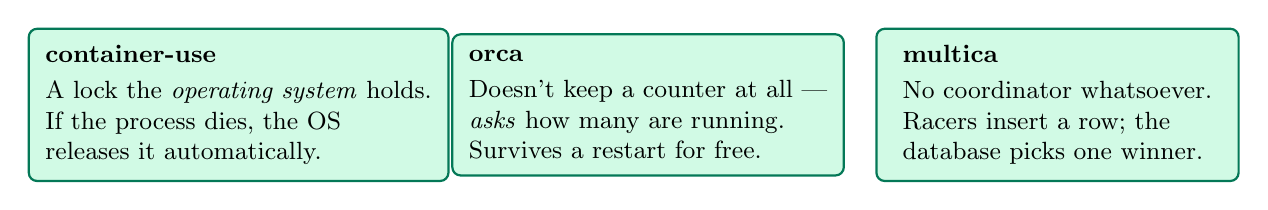
\begin{tikzpicture}[x=1cm,y=1cm]
  \node[greenbox, minimum width=4.6cm, align=left] at (0.2,0)
    {\bfseries container-use\\[2pt]\small A lock the \emph{operating system} holds.\\\small If the process dies, the OS\\\small releases it automatically.};
  \node[greenbox, minimum width=4.6cm, align=left] at (5.4,0)
    {\bfseries orca\\[2pt]\small Doesn't keep a counter at all ---\\\small \emph{asks} how many are running.\\\small Survives a restart for free.};
  \node[greenbox, minimum width=4.6cm, align=left] at (10.6,0)
    {\bfseries multica\\[2pt]\small No coordinator whatsoever.\\\small Racers insert a row; the\\\small database picks one winner.};
\end{tikzpicture}
\end{center}

multica's version is the elegant one and it is worth a sentence, because
\shout{mcgyvr already does exactly this one level up}: claiming a lane is just
creating a branch on the server, and two agents racing for the same branch name
means exactly one wins. Same trick, already in the building.

\newpage
% =====================================================================
\section{So what should you actually do?}

Four decisions, in the order I'd take them. None is a big build.

\begin{center}
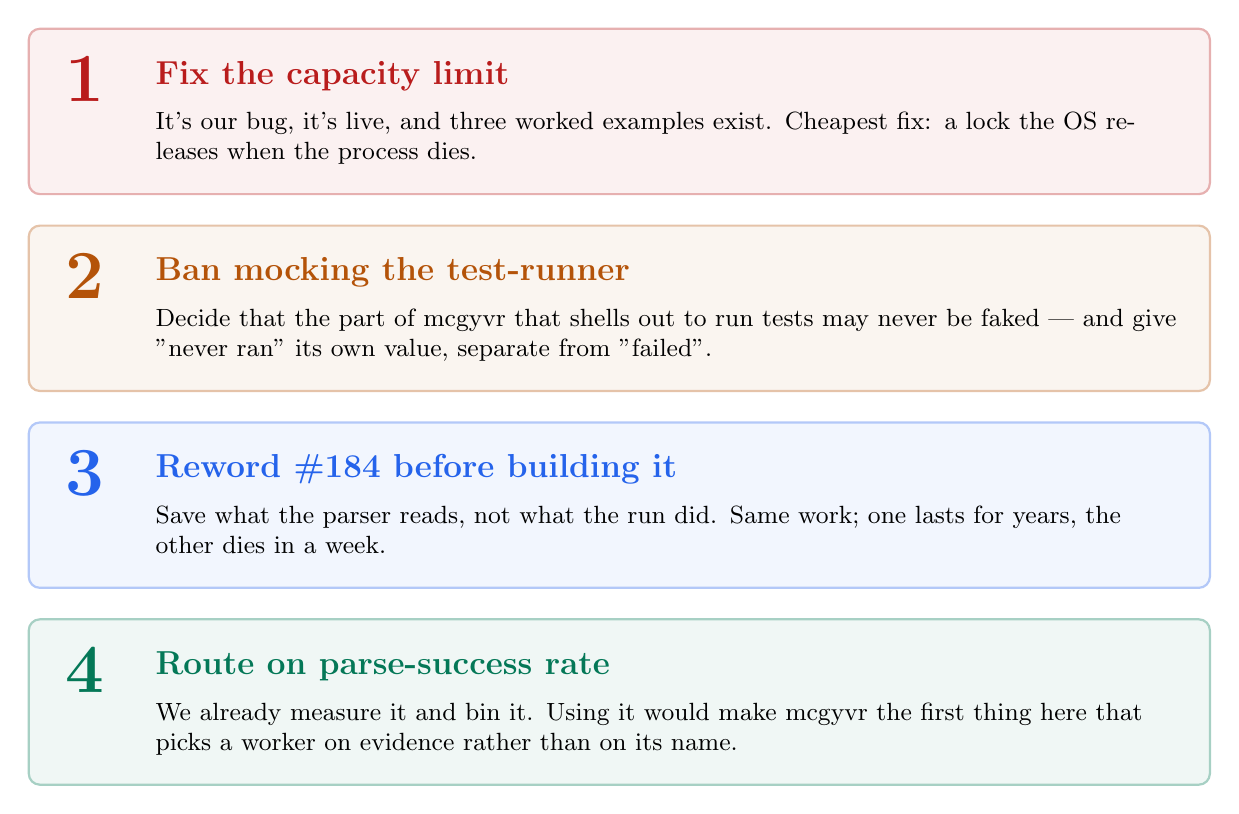
\begin{tikzpicture}[x=1cm,y=1cm]
  \foreach \i/\y/\t/\d/\col in {
    1/0/{Fix the capacity limit}/{It's our bug, it's live, and three worked examples exist. Cheapest fix: a lock the OS releases when the process dies.}/bad,
    2/-2.5/{Ban mocking the test-runner}/{Decide that the part of mcgyvr that shells out to run tests may never be faked --- and give "never ran" its own value, separate from "failed".}/warn,
    3/-5.0/{Reword \#184 before building it}/{Save what the parser reads, not what the run did. Same work; one lasts for years, the other dies in a week.}/accent,
    4/-7.5/{Route on parse-success rate}/{We already measure it and bin it. Using it would make mcgyvr the first thing here that picks a worker on evidence rather than on its name.}/good} {
    \node[anchor=north west, minimum width=15cm, minimum height=2.1cm,
          rounded corners=4pt, fill=\col!6, draw=\col!35, thick] at (0,\y) {};
    \node[anchor=north west] at (0.35,\y-0.25) {\fontsize{26}{26}\selectfont\bfseries\color{\col}\i};
    \node[anchor=north west, font=\large\bfseries\color{\col}] at (1.5,\y-0.3) {\t};
    \node[anchor=north west, text width=13.1cm, font=\small, align=left] at (1.5,\y-0.95) {\d};
  }
\end{tikzpicture}
\end{center}

\vspace{4pt}

\begin{keybox}{Two things I want to be straight about}
\shout{Nothing has been filed.} The review documents these four; turning them into
issues is your call, not mine.

\medskip
\shout{Half the review has not been double-checked.} Six independent readers
re-checked repositories 6--10. Four of those six found real errors in the first
pass --- and \emph{every single error pointed the same way}, making the other
projects look less capable than they are. Repositories 1--5 have had no second
reading. The honest assumption is that they contain the same kind of error, in
the same direction.
\end{keybox}

\vspace{6pt}

\begin{plainbox}
\shout{Where everything lives.} Full review:
\code{docs/prior-art-review-2026-08-06.md} on branch \code{lane/175} --- 1,305
lines, every claim carrying the exact commit it came from so anyone who doesn't
believe it can go and check. No pull request has been opened, and nothing in it
has been reviewed by you yet.
\end{plainbox}

\end{document}
